\documentclass[tikz,border=10pt]{standalone}
\usepackage[T1]{fontenc}
\usepackage{tgheros}
\usepackage{sfmath}
\usepackage{amsmath}
\usepackage{tikz}
\usetikzlibrary{arrows.meta,positioning,shapes.geometric,fit,backgrounds,calc,patterns}
\usepackage{xcolor}

\renewcommand{\familydefault}{\sfdefault}

% Academic Semantic Palette (Harvard Crimson & ETH Zurich)
\definecolor{ethdarkblue}{HTML}{1F407A}
\definecolor{ethblue}{HTML}{215CAF}
\definecolor{ethbronze}{HTML}{B87333}
\definecolor{ethpurple}{HTML}{5B4B8A}
\definecolor{harvardcrimson}{HTML}{A51C30}
\definecolor{ethslate}{HTML}{334155}
\definecolor{gridgray}{HTML}{E2E8F0}
\definecolor{safegreen}{HTML}{0D9488}
\definecolor{dangerred}{HTML}{DC2626}

% Stage Colors
\definecolor{colTrans}{HTML}{0284C7}     % Light Blue
\definecolor{colDMA}{HTML}{0EA5E9}       % Sky Blue
\definecolor{colPerc}{HTML}{2563EB}      % Royal Blue
\definecolor{colPolicy}{HTML}{D97706}    % Amber / Bronze
\definecolor{colIPC}{HTML}{7C3AED}       % Violet
\definecolor{colEnforce}{HTML}{059669}   % Emerald
\definecolor{colAct}{HTML}{DC2626}       % Crimson

\begin{document}
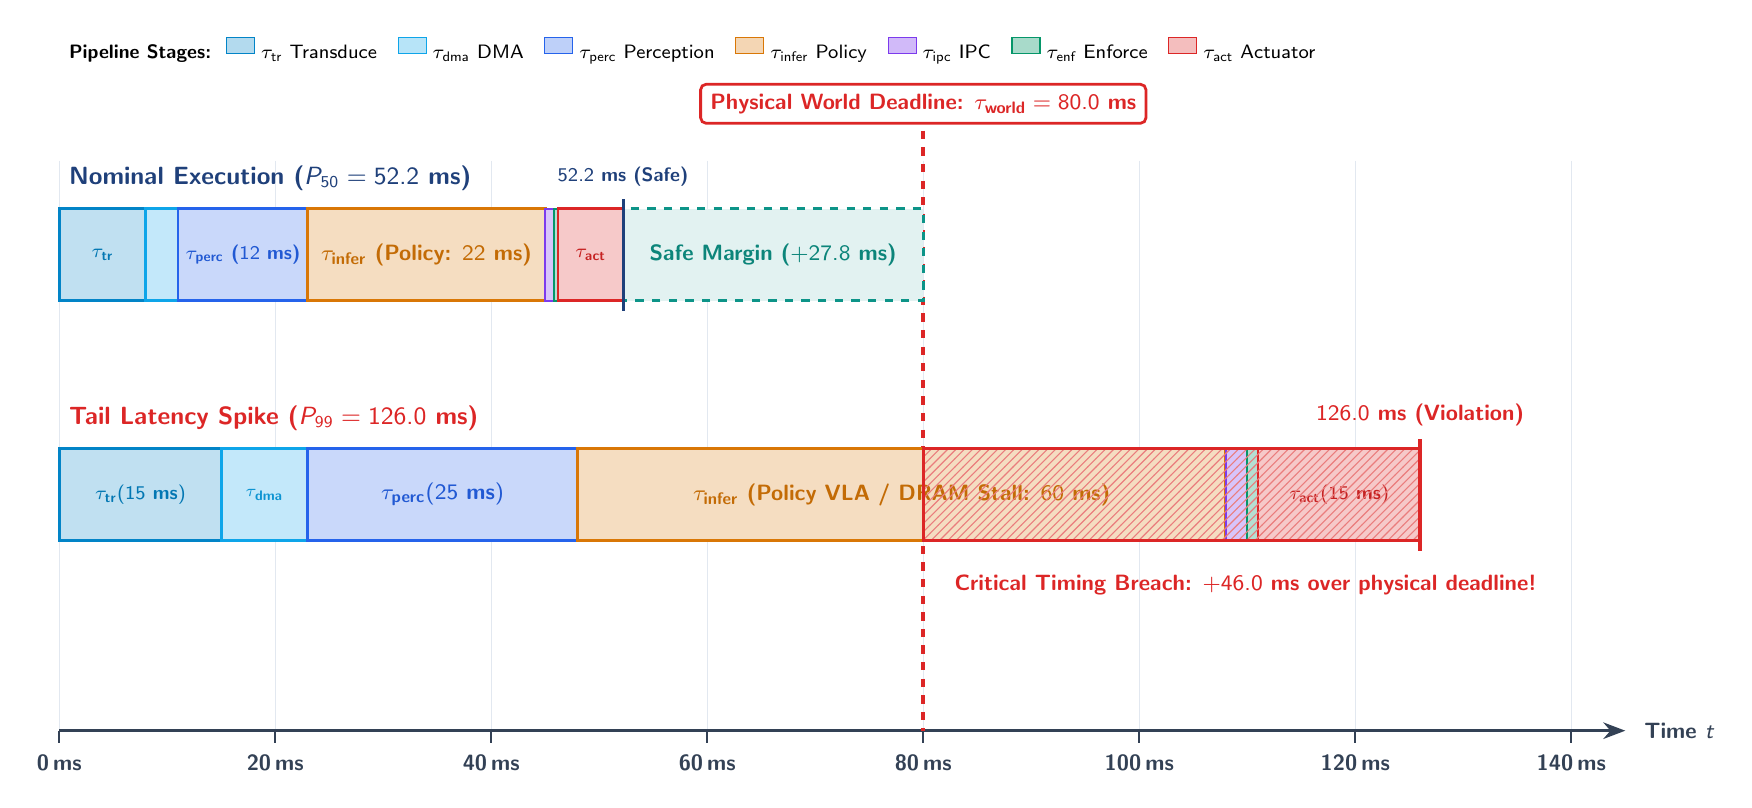
\begin{tikzpicture}[
  font=\sffamily,
  >=Stealth,
  scale=1.0
]

  % ---------------------------------------------------------------------------
  % PARAMETERS: Time Scale 1 ms = 0.054 in (140 ms = 7.56 in)
  % ---------------------------------------------------------------------------
  \def\xscale{0.054in}
  \def\yNom{0.0in}
  \def\yTail{-1.20in}
  \def\yAxis{-2.15in}
  \def\barH{0.46in}

  % ---------------------------------------------------------------------------
  % BACKGROUND GRID & TIME AXIS
  % ---------------------------------------------------------------------------
  \foreach \t in {0, 20, 40, 60, 80, 100, 120, 140} {
    \draw[gridgray, line width=0.5pt] (\t*\xscale, 0.70in) -- (\t*\xscale, \yAxis);
    \draw[ethslate, line width=0.8pt] (\t*\xscale, \yAxis) -- (\t*\xscale, \yAxis - 0.06in);
    \node[font=\fontsize{8pt}{10pt}\selectfont\bfseries, text=ethslate, below=1pt] at (\t*\xscale, \yAxis - 0.06in) {\t\,ms};
  }

  % Time Axis line
  \draw[->, ethslate, line width=1.1pt] (0, \yAxis) -- (145*\xscale, \yAxis)
    node[right=3pt, font=\fontsize{8.5pt}{11pt}\selectfont\bfseries, text=ethslate] {Time $t$};

  % ---------------------------------------------------------------------------
  % PHYSICAL WORLD DEADLINE (t = 80 ms)
  % ---------------------------------------------------------------------------
  \draw[dangerred, dashed, line width=1.5pt] (80*\xscale, 0.85in) -- (80*\xscale, \yAxis);
  \node[draw=dangerred, fill=white, line width=1pt, rounded corners=2pt, inner sep=3.5pt, font=\fontsize{8pt}{10pt}\selectfont\bfseries, text=dangerred, anchor=south] at (80*\xscale, 0.88in) {
    Physical World Deadline: $\tau_{\text{world}} = 80.0\text{ ms}$
  };

  % ---------------------------------------------------------------------------
  % TRACK 1: NOMINAL SENSE-TO-ACTUATION PATH (P50 = 52.2 ms)
  % ---------------------------------------------------------------------------
  \node[anchor=south west, font=\fontsize{9pt}{11.5pt}\selectfont\bfseries, text=ethdarkblue] at (0, 0.50in) {
    Nominal Execution ($P_{50} = 52.2\text{ ms}$)
  };

  % Segments: 
  % 1. Transduce (8 ms: 0 -> 8)
  \draw[fill=colTrans!25, draw=colTrans, line width=0.9pt] (0, \yNom) rectangle ++(8*\xscale, \barH)
    node[midway, font=\fontsize{7pt}{8.5pt}\selectfont\bfseries, text=colTrans!90!black] {$\tau_{\text{tr}}$};

  % 2. DMA Ingest (3 ms: 8 -> 11)
  \draw[fill=colDMA!25, draw=colDMA, line width=0.9pt] (8*\xscale, \yNom) rectangle ++(3*\xscale, \barH);

  % 3. Perception (12 ms: 11 -> 23)
  \draw[fill=colPerc!25, draw=colPerc, line width=0.9pt] (11*\xscale, \yNom) rectangle ++(12*\xscale, \barH)
    node[midway, font=\fontsize{7.5pt}{9pt}\selectfont\bfseries, text=colPerc!90!black] {$\tau_{\text{perc}}$ ($12\text{ ms}$)};

  % 4. Policy (22 ms: 23 -> 45)
  \draw[fill=colPolicy!25, draw=colPolicy, line width=0.9pt] (23*\xscale, \yNom) rectangle ++(22*\xscale, \barH)
    node[midway, font=\fontsize{8pt}{10pt}\selectfont\bfseries, text=colPolicy!90!black] {$\tau_{\text{infer}}$ (Policy: $22\text{ ms}$)};

  % 5. IPC (0.8 ms: 45 -> 45.8)
  \draw[fill=colIPC!30, draw=colIPC, line width=0.6pt] (45*\xscale, \yNom) rectangle ++(0.8*\xscale, \barH);

  % 6. Enforce (0.4 ms: 45.8 -> 46.2)
  \draw[fill=colEnforce!30, draw=colEnforce, line width=0.6pt] (45.8*\xscale, \yNom) rectangle ++(0.4*\xscale, \barH);

  % 7. Actuator Rise (6.0 ms: 46.2 -> 52.2)
  \draw[fill=colAct!25, draw=colAct, line width=0.9pt] (46.2*\xscale, \yNom) rectangle ++(6*\xscale, \barH)
    node[midway, font=\fontsize{7pt}{8.5pt}\selectfont\bfseries, text=colAct!90!black] {$\tau_{\text{act}}$};

  % Safe Margin Bracket (52.2 -> 80.0 ms)
  \draw[fill=safegreen!12, draw=safegreen, dashed, line width=1.0pt] (52.2*\xscale, \yNom) rectangle ++(27.8*\xscale, \barH)
    node[midway, font=\fontsize{8pt}{10pt}\selectfont\bfseries, text=safegreen!90!black] {
      Safe Margin ($+27.8\text{ ms}$)
    };

  % Nominal End Marker
  \draw[ethdarkblue, line width=1.1pt] (52.2*\xscale, \yNom - 0.05in) -- (52.2*\xscale, \yNom + \barH + 0.05in);
  \node[font=\fontsize{7.5pt}{9.5pt}\selectfont\bfseries, text=ethdarkblue, above=1pt] at (52.2*\xscale, \yNom + \barH + 0.05in) {
    $52.2\text{ ms}$ (Safe)
  };

  % ---------------------------------------------------------------------------
  % TRACK 2: TAIL LATENCY PATH (P99 = 126.0 ms)
  % ---------------------------------------------------------------------------
  \node[anchor=south west, font=\fontsize{9pt}{11.5pt}\selectfont\bfseries, text=dangerred] at (0, \yTail + 0.50in) {
    Tail Latency Spike ($P_{99} = 126.0\text{ ms}$)
  };

  % Segments:
  % 1. Transduce (15 ms: 0 -> 15)
  \draw[fill=colTrans!25, draw=colTrans, line width=0.9pt] (0, \yTail) rectangle ++(15*\xscale, \barH)
    node[midway, font=\fontsize{7.5pt}{9pt}\selectfont\bfseries, text=colTrans!90!black] {$\tau_{\text{tr}} (15\text{ ms})$};

  % 2. DMA Ingest (8 ms: 15 -> 23)
  \draw[fill=colDMA!25, draw=colDMA, line width=0.9pt] (15*\xscale, \yTail) rectangle ++(8*\xscale, \barH)
    node[midway, font=\fontsize{6.5pt}{8pt}\selectfont\bfseries, text=colDMA!90!black] {$\tau_{\text{dma}}$};

  % 3. Perception (25 ms: 23 -> 48)
  \draw[fill=colPerc!25, draw=colPerc, line width=0.9pt] (23*\xscale, \yTail) rectangle ++(25*\xscale, \barH)
    node[midway, font=\fontsize{8pt}{10pt}\selectfont\bfseries, text=colPerc!90!black] {$\tau_{\text{perc}} (25\text{ ms})$};

  % 4. Policy (60 ms: 48 -> 108)
  \draw[fill=colPolicy!25, draw=colPolicy, line width=0.9pt] (48*\xscale, \yTail) rectangle ++(60*\xscale, \barH)
    node[midway, font=\fontsize{8.5pt}{10.5pt}\selectfont\bfseries, text=colPolicy!90!black] {$\tau_{\text{infer}}$ (Policy VLA / DRAM Stall: $60\text{ ms}$)};

  % 5. IPC (2 ms: 108 -> 110)
  \draw[fill=colIPC!30, draw=colIPC, line width=0.7pt] (108*\xscale, \yTail) rectangle ++(2*\xscale, \barH);

  % 6. Enforce (1 ms: 110 -> 111)
  \draw[fill=colEnforce!30, draw=colEnforce, line width=0.7pt] (110*\xscale, \yTail) rectangle ++(1*\xscale, \barH);

  % 7. Actuator Rise (15 ms: 111 -> 126)
  \draw[fill=colAct!25, draw=colAct, line width=0.9pt] (111*\xscale, \yTail) rectangle ++(15*\xscale, \barH)
    node[midway, font=\fontsize{7.5pt}{9pt}\selectfont\bfseries, text=colAct!90!black] {$\tau_{\text{act}} (15\text{ ms})$};

  % Timing Breach Overlay Hatch (80 -> 126 ms)
  \draw[pattern=north east lines, pattern color=dangerred!60, draw=dangerred, line width=1.1pt] 
    (80*\xscale, \yTail) rectangle (126*\xscale, \yTail + \barH);

  % Breach Callout Text
  \node[font=\fontsize{8.5pt}{10.5pt}\selectfont\bfseries, text=dangerred, anchor=west] at (82*\xscale, \yTail - 0.22in) {
    Critical Timing Breach: $+46.0\text{ ms}$ over physical deadline!
  };

  % Tail End Marker
  \draw[dangerred, line width=1.2pt] (126*\xscale, \yTail - 0.05in) -- (126*\xscale, \yTail + \barH + 0.05in);
  \node[font=\fontsize{8pt}{10pt}\selectfont\bfseries, text=dangerred, above=1pt] at (126*\xscale, \yTail + \barH + 0.05in) {
    $126.0\text{ ms}$ (Violation)
  };

  % ---------------------------------------------------------------------------
  % LEGEND (Top row of clean semantic pills)
  % ---------------------------------------------------------------------------
  \coordinate (L0) at (0, 1.25in);
  \node[anchor=west, font=\fontsize{7.5pt}{9.5pt}\selectfont] at (L0) {
    \textbf{Pipeline Stages:}\;
    \tikz[baseline=-2pt]{\draw[fill=colTrans!30, draw=colTrans] (0,0) rectangle (0.14in, 0.08in);}\;$\tau_{\text{tr}}$ Transduce\quad
    \tikz[baseline=-2pt]{\draw[fill=colDMA!30, draw=colDMA] (0,0) rectangle (0.14in, 0.08in);}\;$\tau_{\text{dma}}$ DMA\quad
    \tikz[baseline=-2pt]{\draw[fill=colPerc!30, draw=colPerc] (0,0) rectangle (0.14in, 0.08in);}\;$\tau_{\text{perc}}$ Perception\quad
    \tikz[baseline=-2pt]{\draw[fill=colPolicy!30, draw=colPolicy] (0,0) rectangle (0.14in, 0.08in);}\;$\tau_{\text{infer}}$ Policy\quad
    \tikz[baseline=-2pt]{\draw[fill=colIPC!35, draw=colIPC] (0,0) rectangle (0.14in, 0.08in);}\;$\tau_{\text{ipc}}$ IPC\quad
    \tikz[baseline=-2pt]{\draw[fill=colEnforce!35, draw=colEnforce] (0,0) rectangle (0.14in, 0.08in);}\;$\tau_{\text{enf}}$ Enforce\quad
    \tikz[baseline=-2pt]{\draw[fill=colAct!30, draw=colAct] (0,0) rectangle (0.14in, 0.08in);}\;$\tau_{\text{act}}$ Actuator
  };

\end{tikzpicture}
\end{document}
